\section{Abundance calibrations and radial decrements}
\label{sec:abund_meas_grad_dec}

We measure gas-phase metallicities of individual MaNGA spaxels using the ratios between the fluxes of strong nebular emission lines, since the ``direct" ($T_e$) method requires much deeper spectroscopy at the high expected metallicities of MaNGA spaxels. We rely on one of the strong-line calibrations of \citet[][hereafter, \citetalias{pilyugin_grebel_2016}]{pilyugin_grebel_2016}, which matches several strong-line ratios to $T_e$ abundances over a reference sample of 313 HII regions. Specifically, we use the \texttt{R2} calibration, referred to hereafter as \texttt{PG16-R2}. The three strong-line ratios used to define the calibration in \citetalias{pilyugin_grebel_2016} are defined as follows:

\begin{itemize}
    \item $R_2 = \frac{\rm F([OII]_{3727}) + F([OII]_{3729})}{\rm F(H \beta)}$
    \item $R_3 = \frac{\rm F([OIII]_{4959}) + F([OIII]_{5007})}{\rm F(H \beta)}$
    \item $N_2 = \frac{\rm F([NII]_{6548}) + F([NII]_{6584})}{\rm F(H \beta)}$
\end{itemize}

Generally, the strong-line ratios $R_2$ \& $R_3$ (as well as their sum, generally notated $R_{23}$), are double-valued; that is, a single value can indicate one of two values of oxygen abundance. In the \texttt{PG16-R2} calibration, this degeneracy between ``upper" and ``lower" branches is broken using the $N_2$ ratio (previous work has cautioned against using nitrogen-based line ratios to determine oxygen abundance, because the abundance ratio of N/O is variable, even at fixed oxygen abundance---but adopting it for the coarse task of deciding the $R_{23}$ branch is safer). The accuracy of the resulting oxygen abundance estimate is $\lesssim 0.1~{\rm dex}$ over the range $7.0 \le 12 + \log{\frac{O}{H}} \le 9.0$, and \citet{schaefer_19_ohno} has found the \texttt{PG16-R2} calibration to be less susceptible to N/O variations than other strong-line calibrations. Since variations in excitation (ionization parameter) can impact reliability of abundance estimates, this calibration adjusts for this effect using the ratio between $R_2$ \& $R_3$. \citep{pilyugin_grebel_2018_manga} concluded that for MaNGA spectra, the \texttt{PG16-R2} calibration does not suffer from the same excitation-dependent deficiencies that purely $N_2$-dependent calibrations do.

The metallicity for a particular spaxel is estimated according to a Monte Carlo randomization of attenuation-corrected emission-lines. The first four Balmer emission lines (\ha, \hb, \hg, \hd) are used to estimate the attenuation law, assuming a \citet{charlot_fall_00} two-component dust model. The best-fitting dust parameters $\tau_V$ and $\mu$ (along with their covariances) are found through Levenberg-Marquardt optimization. The line-specific attenuation correction-factors are then randomized according to the covariance matrix of the best-fit parameters, with 1000 draws total. The observed emission-line fluxes are likewise independently resampled 1000 times according to their reported uncertainties, and multiplied with the resampled dust-corrections. The combination of these draws for all emission lines is used to approximate the distribution of possible strong-line ratios $R_2$, $R_3$, and $N_2$, which themselves are used to approximate draws from the distribution of oxygen abundance. This process is repeated for each spaxel in the field of view. The median of those 1000 draws from the oxygen abundance distribution is taken as the fiducial oxygen abundance for a spaxel, \met; with the median absolute deviation of that distribution is taken as a measure of the dispersion. Both are are logarithmic quantities.

\subsection{Radial decrement definition}
\label{subsec:bintervals}

Since the star-forming disk is the main engine driving galaxy chemical evolution, the most useful radial unit is a \emph{disk effective radius} ($R_e^d$) rather than a \emph{total effective radius} ($R_e^t$). We use the bulge-disk decompositions from the MaNGA PyMorph photometric catalog \citep{fischer_2019_pymorph} to assign a radial coordinate to all spaxels based on the measured disk effective radius (hereafter, the shorthand $R_e$ refers to a disk effective radius, unless otherwise specified). In practice, radial oxygen abundance trends fitted to ensembles of individual spaxels tend to be dictated strongly by the measurements in the outermost $\sim 0.5 R_e$, since the number of spaxels within a radial interval rises in proportion to the distance from the center of the galaxy. For the case of an abundance gradient with non-constant slope, the central abundance would also be improperly estimated. In \citet{belfiore_2017_manga-metgrad}, metallicity measurements were binned in intervals of 0.1 $R_e$ and an unweighted least-squares fit made, thereby standardizing the contribution at various radii to the gradient fit. Instead, we define a radial metallicity ``decrement" between two widely-spaced annuli, as $\Delta_{in}^{out} = \met_{in} - \met_{out}$; in other words, a positive decrement indicates that oxygen abundance decreases radially.

The bounds for the radial bins are chosen to minimize the adverse effects of blurring by the PSF. We exclude spaxels along or close to the minor axes of inclined galaxies, where the PSF-induced smoothing in the data will ``smear out" radial variations most severely: galaxies with observed minor-to-major axis ratios under 0.33 are excluded entirely, since dust-correction becomes extremely problematic at inclinations greater than 75 deg \citep{pellegrini_2019_warpfield}. At axis ratios greater than 0.75, it is difficult to accurately determine a galaxy's axis ratio, and so all spaxels are included. In the intermediate range ($0.33 < b/a < 0.75$), the azimuthal angle from the major axis determines the acceptance or rejection of a spaxel, with the angle rising linearly from 20 degrees at $b/a = 0.33$ to 90 degrees (i.e., no restriction) at $b/a = 0.75$.

\begin{figure*}
    \centering
    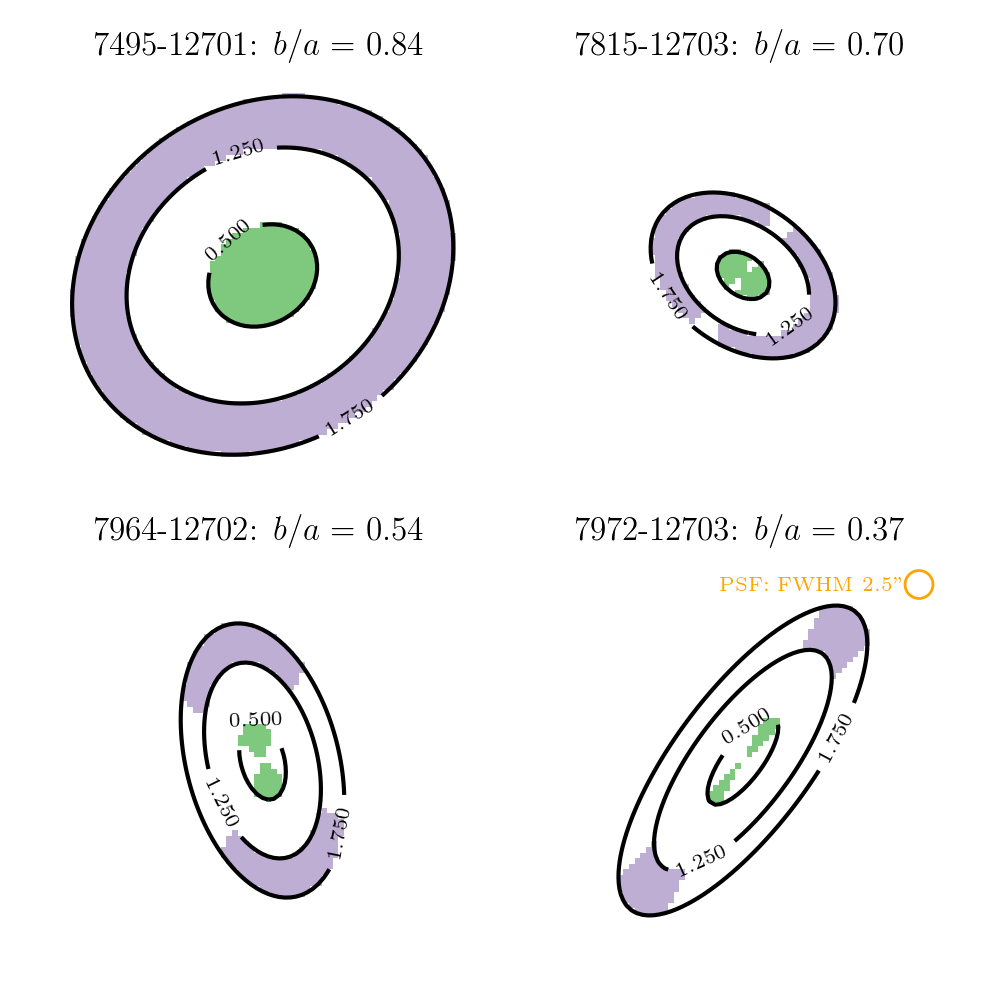
\includegraphics[width=5 in]{radial_bins}
    \caption[An illustration of the radial binning scheme used to compute radial metallicity decrements, along with azimuthal cuts excluding the minor axis.]{The radial binning scheme described above, applied to four MaNGA galaxies with decreasing disk aspect-ratios. Pixels are colored according to their use in radial bins: light green indicates radial bin 0 ($0.0 - 0.5~R_e$), and lavender indicates radial bin 1 ($1.25-1.75~R_e$). Pixels colored white indicate locations not included in any bin, due to either radial coordinate or azimuthal angle away from the major axis. These restrictions are applied in addition to those on data-quality (see Section \ref{subsubsec:data_quality}). Contours are in units of $R_e$, and are labeled at the outer boundary of bin 0, as well as the inner \& outer boundaries of bin 1. The spatial resolution element (FWHM) is visualized as an orange circle in the bottom-right panel: as inclination increases, the PSF samples an increasing diversity of galaxy radii along the minor axis.}
    \label{fig:radial_bins}
\end{figure*}

Though we might desire to maximize the number of radial bins available, there is limited utility to reducing bin width smaller than the PSF size. Furthermore, a larger radial interval allows more spaxels to be aggregated. Most important for our purposes is the observation that both the MaNGA Primary and Secondary samples are relatively clean from PSF-induced contamination at radial separations greater than $0.5~R_e$. We elect to use radial bins with widths of $0.5~R_e$, and spaced apart by $0.75~R_e$ (see Figure \ref{fig:radial_bins}). In this work, we consider bin limits of [0.0, 0.5] $R_e$ (radial bin 0) and [1.25, 1.75] $R_e$ (radial bin 1).

\subsection{Sample \& Data quality}
\label{subsubsec:data_quality}

Our base sample of galaxies is the PyMorph VAC (4266 galaxies), almost all of which have total stellar masses from the MaNGA-PCA VAC. Of these, 1152 (2080) have \hi mass estimates (upper-limits) from either targeted GBT follow-up \citep{masters_19_himanga, goddy_2020_gbtcal}, ALFALFA \citep{haynes_2018_alfalfa}, or GASS/GASS-low \citep{catinella_2010_GASS}, accessed in that descending order of priority. 

We adopt the following constraints on individual spaxels within galaxies, all of which must be met in order for the spaxel to be included in the radial fits and decrement calculation. These cuts are applied in addition to the radial and azimuthal restrictions described above.

\begin{itemize}
    \item Signal-to-noise cuts: We require $S/N(\ha) > 5$, $S/N(\hb) > 3$, $S/N([{\rm O ~ III}]) > 3$, and $S/N([{\rm N ~ II}]) > 3$, since these lines form the basis for the selection of star-formation-dominated spaxels.
    \item Excitation cuts: We requires spaxels to lie in the star-formation-dominated portion of the $[{\rm N ~ II}] / \ha$-versus-$[{\rm O ~ III}] / \hb$ excitation diagram, i.e., below the \citet{kauffmann_03_agn} and \citet{kewley_dopita_01} demarcation lines.
    \item Diffuse ionized gas (DIG) rejection: \citet{lacerda_2018_califa_dig} finds that when EW(\ha) is less than 3$\mbox{\AA}$, DIG dominates the emission spectrum. We select only spaxels with $EW(\ha) \ge 3 {\rm \AA}$.
    \item Restrictions on resampled oxygen abundances: The Monte Carlo-resampled distribution of the oxygen abundance (obtained from the line-ratio calibration) must have a median absolute deviation (MAD) $< 0.3 ~ {\rm dex}$, and must lie in the range [7.0, 9.0] (where the \texttt{PG16-R2} calibration is well-characterized).
\end{itemize}

In order for an individual galaxy to be included for the purposes of radial metallicity trends, there must be at least 8 (10) unmasked spaxels in radial bin 0 (radial bin 1). With these thresholds set, we are left with 252 (110) galaxies having \hi masses (upper-limits). A further 273 galaxies passing all spectroscopic data-quality criteria above (bullet-points), but which were not targeted in the HI follow-up, are included separately.